%%%%%%%%%%%%%%%%%%%%%%%%%%%%%%%%%%%%%%%%%%%%%%%%%%%%%%%%%%%%%%%%%%%%%%%%%%%%%%%%%%
\begin{frame}[fragile]\frametitle{}
\begin{center}
{\Large Domain and Task Adaptation}

{\tiny (Ref: Applied LLMs Mastery 2024 - Aishwarya Reganti)}

\end{center}


\end{frame}

%%%%%%%%%%%%%%%%%%%%%%%%%%%%%%%%%%%%%%%%%%%%%%%%%%%%%%%%%%%%%%%%%%%%%%%%%%%%%%%%%%
\begin{frame}[fragile]\frametitle{Using LLMs Effectively}
  \begin{itemize}
    \item General AI models like ChatGPT excel in diverse text generation but may lack depth for specific domains.
    \item They might generate inaccurate or contextually inappropriate content, known as hallucinations.
    \item Task-specific and domain-specific LLMs are crucial for specialized domains, possessing industry-specific knowledge.
    \item Domain-specific LLMs ensure accurate interpretation of specialized terminology and practices.
 
  \end{itemize}
\end{frame}

%%%%%%%%%%%%%%%%%%%%%%%%%%%%%%%%%%%%%%%%%%%%%%%%%%%%%%%%%%%%%%%%%%%%%%%%%%%%%%%%%%
\begin{frame}[fragile]\frametitle{Benefits of Domain-specific LLMs}
  \begin{itemize}
	\item Depth and Precision: Tailored for understanding industry-specific terminology, ensuring precision.
	\item Overcoming Limitations: Excel in accuracy and context relevance, overcoming general LLM limitations.
	\item Enhanced User Experiences: Provide tailored and personalized responses for better user experiences.
	\item Improved Efficiency: Streamline operations, automate tasks, and boost productivity for businesses.
	\item Addressing Privacy Concerns: Ensure data protection and privacy adherence in sensitive industries.
  \end{itemize}
\end{frame}


%%%%%%%%%%%%%%%%%%%%%%%%%%%%%%%%%%%%%%%%%%%%%%%%%%%%%%%%%%%%%%%%%%%%%%%%%%%%%%%%%%
\begin{frame}[fragile]\frametitle{Methods}
  \begin{itemize}
	\item Few Shots prompting
	\item Retrieval Augmented Generation
	\item Domain Specific pre-training (ie full, from scratch on own data)
	\item Domain Specific fine-tuning (with change in weights or additional adopter weights)
  \end{itemize}

		\begin{center}
		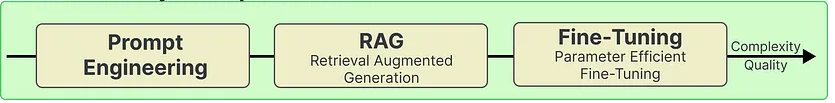
\includegraphics[width=\linewidth,keepaspectratio]{finetune1}
		\end{center}

{\tiny (Ref: 3 Easy Methods For Improving Your Large Language Model - Towards Data Science - Maarten Grootendorst)}

\end{frame}

%%%%%%%%%%%%%%%%%%%%%%%%%%%%%%%%%%%%%%%%%%%%%%%%%%%%%%%%%%%%%%%%%%%%%%%%%%%%%%%%%%
\begin{frame}[fragile]\frametitle{Example-based Prompt Engineering}


		\begin{center}
		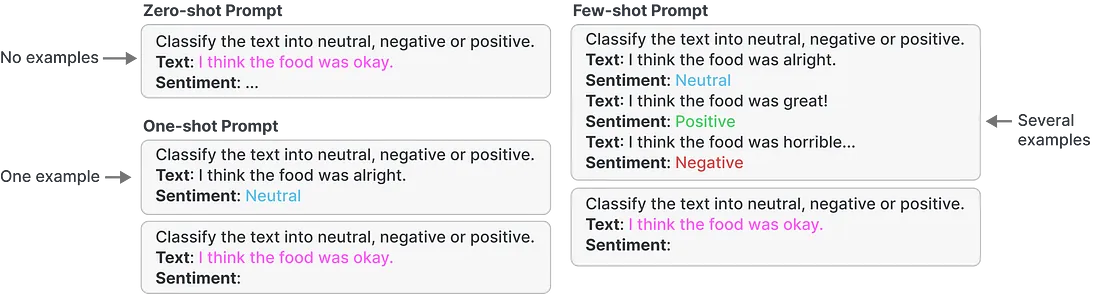
\includegraphics[width=\linewidth,keepaspectratio]{finetune3}
		\end{center}

{\tiny (Ref: 3 Easy Methods For Improving Your Large Language Model - Towards Data Science - Maarten Grootendorst)}

\end{frame}

%%%%%%%%%%%%%%%%%%%%%%%%%%%%%%%%%%%%%%%%%%%%%%%%%%%%%%%%%%%%%%%%%%%%%%%%%%%%%%%%%%
\begin{frame}[fragile]\frametitle{Thoughts-based Prompt Engineering}


		\begin{center}
		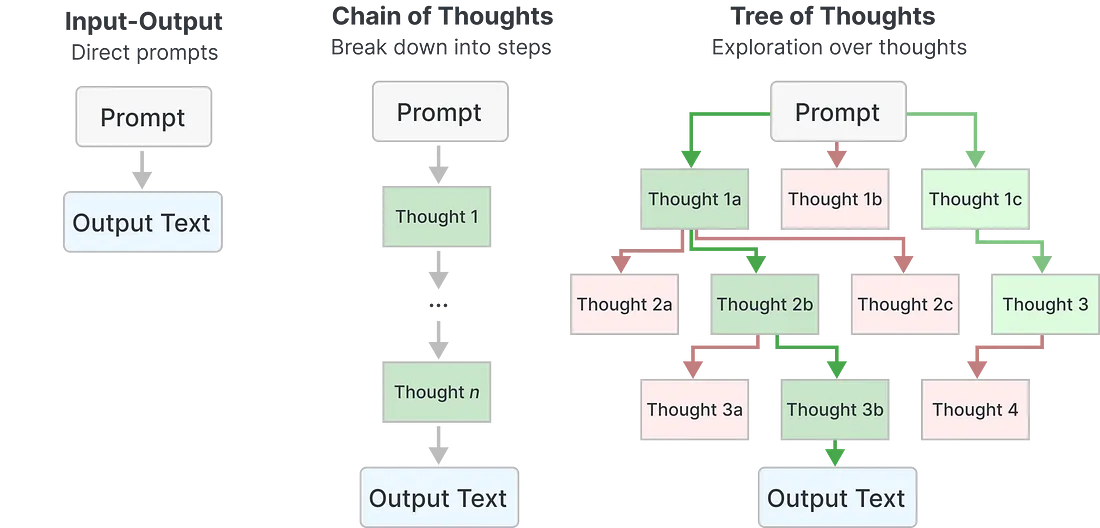
\includegraphics[width=\linewidth,keepaspectratio]{finetune4}
		\end{center}

{\tiny (Ref: 3 Easy Methods For Improving Your Large Language Model - Towards Data Science - Maarten Grootendorst)}

\end{frame}

%%%%%%%%%%%%%%%%%%%%%%%%%%%%%%%%%%%%%%%%%%%%%%%%%%%%%%%%%%%%%%%%%%%%%%%%%%%%%%%%%%
\begin{frame}[fragile]\frametitle{Retrieval Augmented Generation (RAG)}


		\begin{center}
		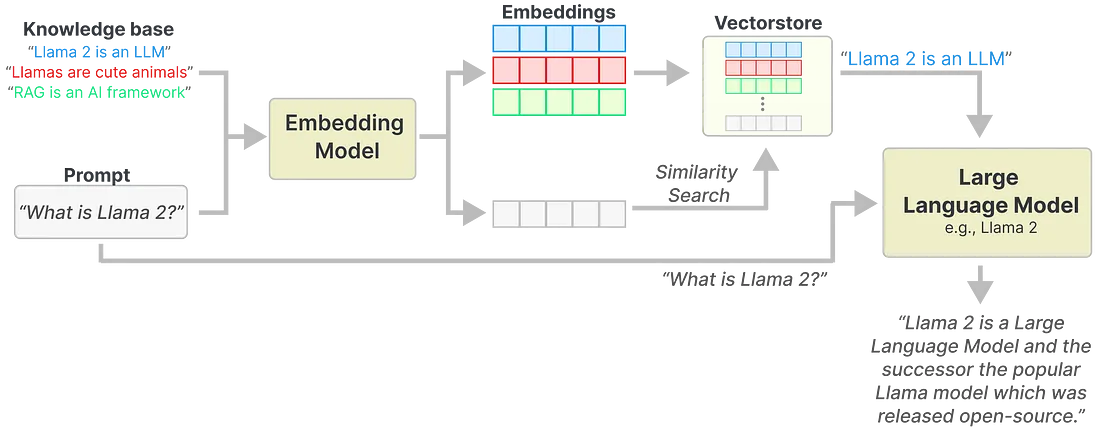
\includegraphics[width=\linewidth,keepaspectratio]{finetune5}
		\end{center}

{\tiny (Ref: 3 Easy Methods For Improving Your Large Language Model - Towards Data Science - Maarten Grootendorst)}

\end{frame}
%%%%%%%%%%%%%%%%%%%%%%%%%%%%%%%%%%%%%%%%%%%%%%%%%%%%%%%%%%%%%%%%%%%%%%%%%%%%%%%%%%
\begin{frame}[fragile]\frametitle{Retrieval Augmented Generation (RAG)}

      \begin{itemize}
        \item Training Duration: Not required.
        \item No model weights; relies on external information retrieval system.
        \item External knowledge provided as context in the prompt.
        \item Advantages: No training costs, low expertise requirement, and easy updating of knowledge base.
      \end{itemize}

\end{frame}


%%%%%%%%%%%%%%%%%%%%%%%%%%%%%%%%%%%%%%%%%%%%%%%%%%%%%%%%%%%
\begin{frame}[fragile]\frametitle{Retrieval Augmented Generation (RAG)}
  \begin{itemize}
    \item \textbf{Definition:} Enhances LLM-generated responses by incorporating up-to-date and contextually relevant information from external sources.
    \item Addresses inconsistency and lack of domain-specific knowledge in LLMs, reducing hallucinations.
    \item \textbf{Two Phases:}
      \begin{enumerate}
        \item Retrieval: Searches and retrieves relevant external information.
        \item Content Generation: LLM synthesizes an answer based on retrieved information and internal training data.
      \end{enumerate}
    \item \textbf{Fundamental RAG Pipeline:}
      \begin{enumerate}
        \item Ingestion: Documents segmented into chunks, embeddings generated, and stored in an index.
        \item Retrieval: System retrieves top-k documents based on embedding similarity.
        \item Synthesis: LLM utilizes contextual knowledge from chunks to formulate accurate responses.
      \end{enumerate}
    \item \textbf{No Training Requirement:} Unlike previous domain adaptation methods, RAG doesn't require model training when specific domain data is provided.
  \end{itemize}
\end{frame}

%%%%%%%%%%%%%%%%%%%%%%%%%%%%%%%%%%%%%%%%%%%%%%%%%%%%%%%%%%%
\begin{frame}[fragile]\frametitle{Retrieval Augmented Generation (RAG)}

\begin{center}
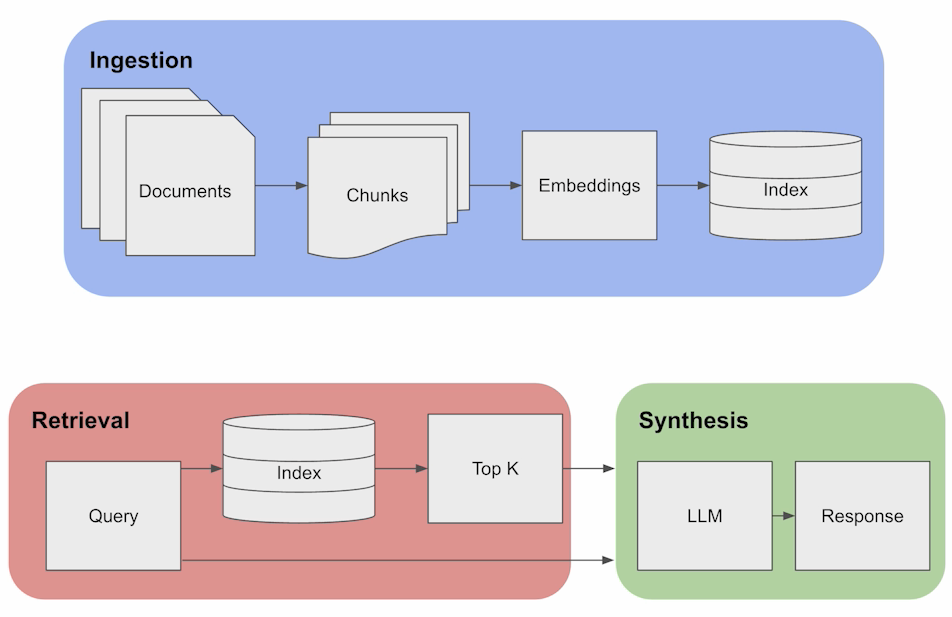
\includegraphics[width=0.8\linewidth,keepaspectratio]{llm125}
\end{center}				

{\tiny (Ref: Applied LLMs Mastery 2024 - Aishwarya Reganti)}

\end{frame}

%%%%%%%%%%%%%%%%%%%%%%%%%%%%%%%%%%%%%%%%%%%%%%%%%%%%%%%%%%%
\begin{frame}[fragile]\frametitle{Retrieval Augmented Generation (RAG)}

\begin{center}
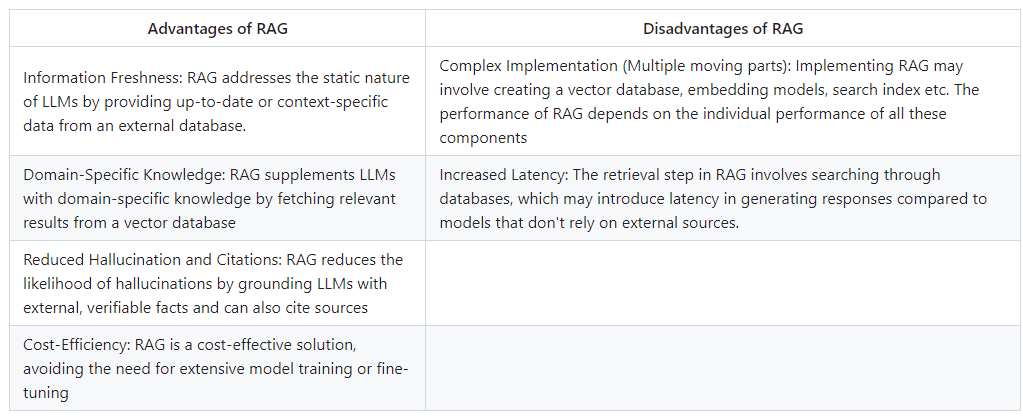
\includegraphics[width=\linewidth,keepaspectratio]{llm126}
\end{center}				

{\tiny (Ref: Applied LLMs Mastery 2024 - Aishwarya Reganti)}

\end{frame}




%%%%%%%%%%%%%%%%%%%%%%%%%%%%%%%%%%%%%%%%%%%%%%%%%%%%%%%%%%%%%%%%%%%%%%%%%%%%%%%%%%
\begin{frame}[fragile]\frametitle{Domain-Specific Pre-Training}

      \begin{itemize}
        \item Training Duration: Days to weeks to months.
        \item Requires extensive domain training data.
        \item Allows customization of model architecture, size, tokenizer, etc.
        \item Examples: PaLM 540B, GPT-3, LLaMA 2.
      \end{itemize}

\end{frame}


%%%%%%%%%%%%%%%%%%%%%%%%%%%%%%%%%%%%%%%%%%%%%%%%%%%%%%%%%%%%%%%%%%%%%%%%%%%%%%%%%%
\begin{frame}[fragile]\frametitle{Domain-Specific Pre-Training}
  \begin{itemize}
    \item \textbf{Definition:} Training large language models on extensive datasets specific to a particular domain.
    \item Aims to enhance understanding and performance within a defined subject area.
    \item \textbf{Example:} BloombergGPT - a 50 billion parameter model designed for finance tasks.
      \begin{itemize}
        \item Financial Sentiment Analysis
        \item Named Entity Recognition
        \item News Classification
        \item Question Answering in Finance
        \item Conversational Systems for Finance
      \end{itemize}
    \item \textbf{Training Data:} FinPile dataset - a mix of domain-specific financial documents and general-purpose text.
    \item Architecture: Based on guidelines, with 70 layers of transformer decoder blocks.
  \end{itemize}
\end{frame}

%%%%%%%%%%%%%%%%%%%%%%%%%%%%%%%%%%%%%%%%%%%%%%%%%%%%%%%%%%%
\begin{frame}[fragile]\frametitle{Domain-Specific Pre-Training}

\begin{center}
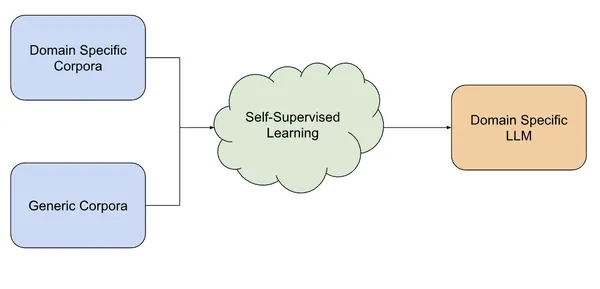
\includegraphics[width=0.8\linewidth,keepaspectratio]{llm124}
\end{center}				

{\tiny (Ref: Applied LLMs Mastery 2024 - Aishwarya Reganti)}

\end{frame}

%%%%%%%%%%%%%%%%%%%%%%%%%%%%%%%%%%%%%%%%%%%%%%%%%%%%%%%%%%%%%%%%%%%%%%%%%%%%%%%%%%
\begin{frame}[fragile]\frametitle{Parameter-Efficient Fine-Tuning}

Instead of fine-tuning the model's billions of parameters, we can leverage PEFT instead, Parameter-Efficient Fine-Tuning. As the name implies, it is a subfield that focuses on efficiently fine-tuning an LLM with as few parameters as possible.

		\begin{center}
		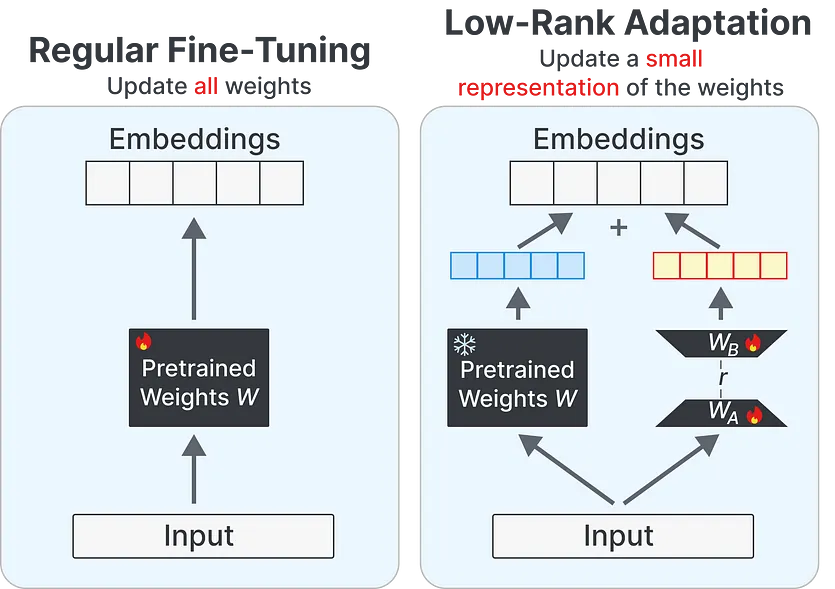
\includegraphics[width=0.6\linewidth,keepaspectratio]{finetune6}
		\end{center}

{\tiny (Ref: 3 Easy Methods For Improving Your Large Language Model - Towards Data Science - Maarten Grootendorst)}

\end{frame}

%%%%%%%%%%%%%%%%%%%%%%%%%%%%%%%%%%%%%%%%%%%%%%%%%%%%%%%%%%%%%%%%%%%%%%%%%%%%%%%%%%
\begin{frame}[fragile]\frametitle{Domain-Specific Fine-Tuning}

      \begin{itemize}
        \item Training Duration: Minutes to hours.
        \item Involves adding domain-specific data and tuning for specific tasks.
        \item Updates the pre-trained LLM model.
        \item Examples: Alpaca, xFinance, ChatDoctor.
      \end{itemize}

\end{frame}

%%%%%%%%%%%%%%%%%%%%%%%%%%%%%%%%%%%%%%%%%%%%%%%%%%%%%%%%%%%
\begin{frame}[fragile]\frametitle{Domain-Specific Fine-Tuning}
  \begin{itemize}
    \item \textbf{Definition:} Refining a pre-existing language model for a specific task or domain.
    \item \textbf{Process:} Fine-tuning a pre-trained general model on domain-specific data for task optimization.
    \item \textbf{Key Steps:}
      \begin{enumerate}
        \item Pre-training: Initial training on an extensive dataset for general language understanding.
        \item Fine-tuning Dataset: Domain-specific dataset tailored to the task.
        \item Fine-tuning Process: Model adjustment based on the new dataset while retaining general understanding.
        \item Task Optimization: Model optimization for specific tasks within the chosen domain.
      \end{enumerate}
    \item \textbf{Advantages:}
      \begin{itemize}
        \item Specialization in a domain for enhanced task effectiveness.
        \item Time and resource savings compared to training from scratch.
        \item Adaptation to specific domain requirements for improved task performance.
      \end{itemize}
    \item \textbf{Example:} ChatDoctor LLM - fine-tuned on Meta-AI's LLaMA using a dataset of patient-doctor dialogues.
  \end{itemize}
\end{frame}

%%%%%%%%%%%%%%%%%%%%%%%%%%%%%%%%%%%%%%%%%%%%%%%%%%%%%%%%%%%%%%%%%%%%%%%%%%%%%%%%%%
\begin{frame}[fragile]\frametitle{Choosing Adaptation Methods}


		\begin{center}
		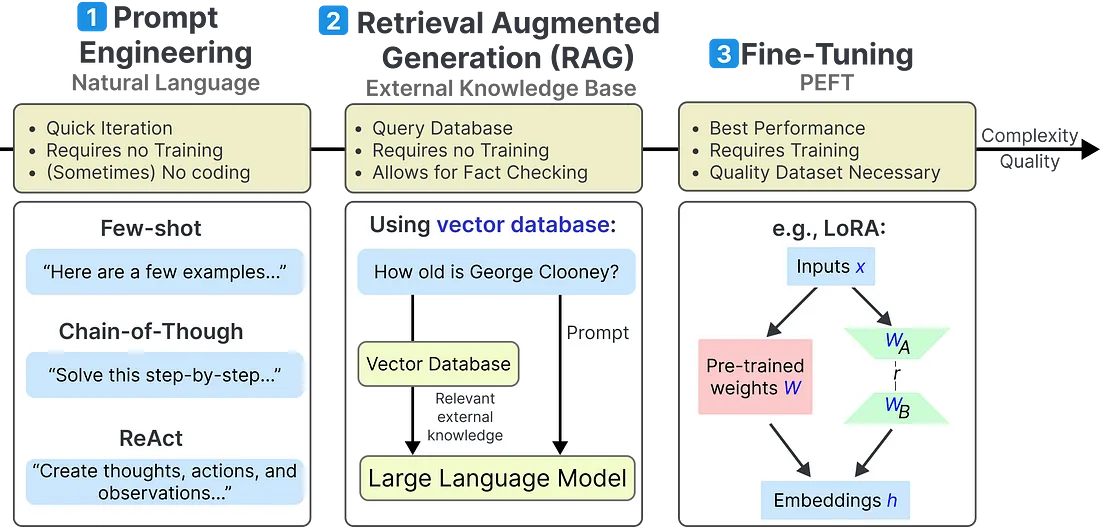
\includegraphics[width=\linewidth,keepaspectratio]{finetune2}
		\end{center}

{\tiny (Ref: 3 Easy Methods For Improving Your Large Language Model - Towards Data Science - Maarten Grootendorst)}

\end{frame}

%%%%%%%%%%%%%%%%%%%%%%%%%%%%%%%%%%%%%%%%%%%%%%%%%%%%%%%%%%%%%%%%%%%%%%%%%%%%%%%%%%
\begin{frame}[fragile]\frametitle{Fine-Tuning Language Models}
  \begin{enumerate}
    \item \textbf{When to Opt for Fine-Tuning?}
      \begin{itemize}
        \item Determine necessity based on task objectives, input-output nature, and success metrics.
        \item Particularly useful for adapting LLMs to new domains with limited data.
      \end{itemize}
    \item \textbf{Data Preparation: Foundation of Success}
      \begin{itemize}
        \item Meticulous data preparation is key for robust fine-tuning.
        \item Identify minimum viable dataset aligning with model complexity for optimal performance.
      \end{itemize}
    \item \textbf{Infrastructure: Backbone of Fine-Tuning}
      \begin{itemize}
        \item Choose efficient infrastructure for GPU access, often provided by cloud services.
        \item Utilize tools like TensorFlow, PyTorch, AWS, GCP, or Anthropic for streamlined processes.
      \end{itemize}
    \item \textbf{Optimization Tactics for Fine-Tuning}
      \begin{itemize}
        \item Start with a smaller base model; use strategies like quantization to minimize size.
        \item Halt training on validation stagnation to prevent overfitting.
        \item Apply transfer learning techniques, e.g., progressively 'unfreezing' layers.
      \end{itemize}
  \end{enumerate}
\end{frame}

%%%%%%%%%%%%%%%%%%%%%%%%%%%%%%%%%%%%%%%%%%%%%%%%%%%%%%%%%%%
\begin{frame}[fragile]\frametitle{Choosing Adaptation Methods}
  \begin{itemize}
    \item \textbf{Domain-Specific Pre-Training:}
      \begin{itemize}
        \item Exclusive Domain Focus: When a model exclusively trained on specific domain data is required.
        \item Customizing Model Architecture: Allows customization of model aspects based on domain requirements.
        \item Extensive Training Data Available: Effective with a large amount of domain-specific training data.
      \end{itemize}
    \item \textbf{Domain-Specific Fine-Tuning:}
      \begin{itemize}
        \item Specialization Needed: Adapting a pre-trained LLM for specific tasks or within a domain.
        \item Task Optimization: Adjusting model parameters for optimal performance in the chosen domain.
        \item Time and Resource Efficiency: Saves time and computational resources compared to training from scratch.
      \end{itemize}
    \item \textbf{RAG (Retrieval Augmented Generation):}
      \begin{itemize}
        \item Information Freshness Matters: Provides up-to-date, context-specific data from external sources.
        \item Reducing Hallucination is Crucial: Grounds LLMs with verifiable facts and citations.
        \item Cost-Efficiency: Implement without extensive model training; avoid fine-tuning.
      \end{itemize}
  \end{itemize}
\end{frame}

%%%%%%%%%%%%%%%%%%%%%%%%%%%%%%%%%%%%%%%%%%%%%%%%%%%%%%%%%%%
\begin{frame}[fragile]\frametitle{Choosing Adaptation Methods}

\begin{center}
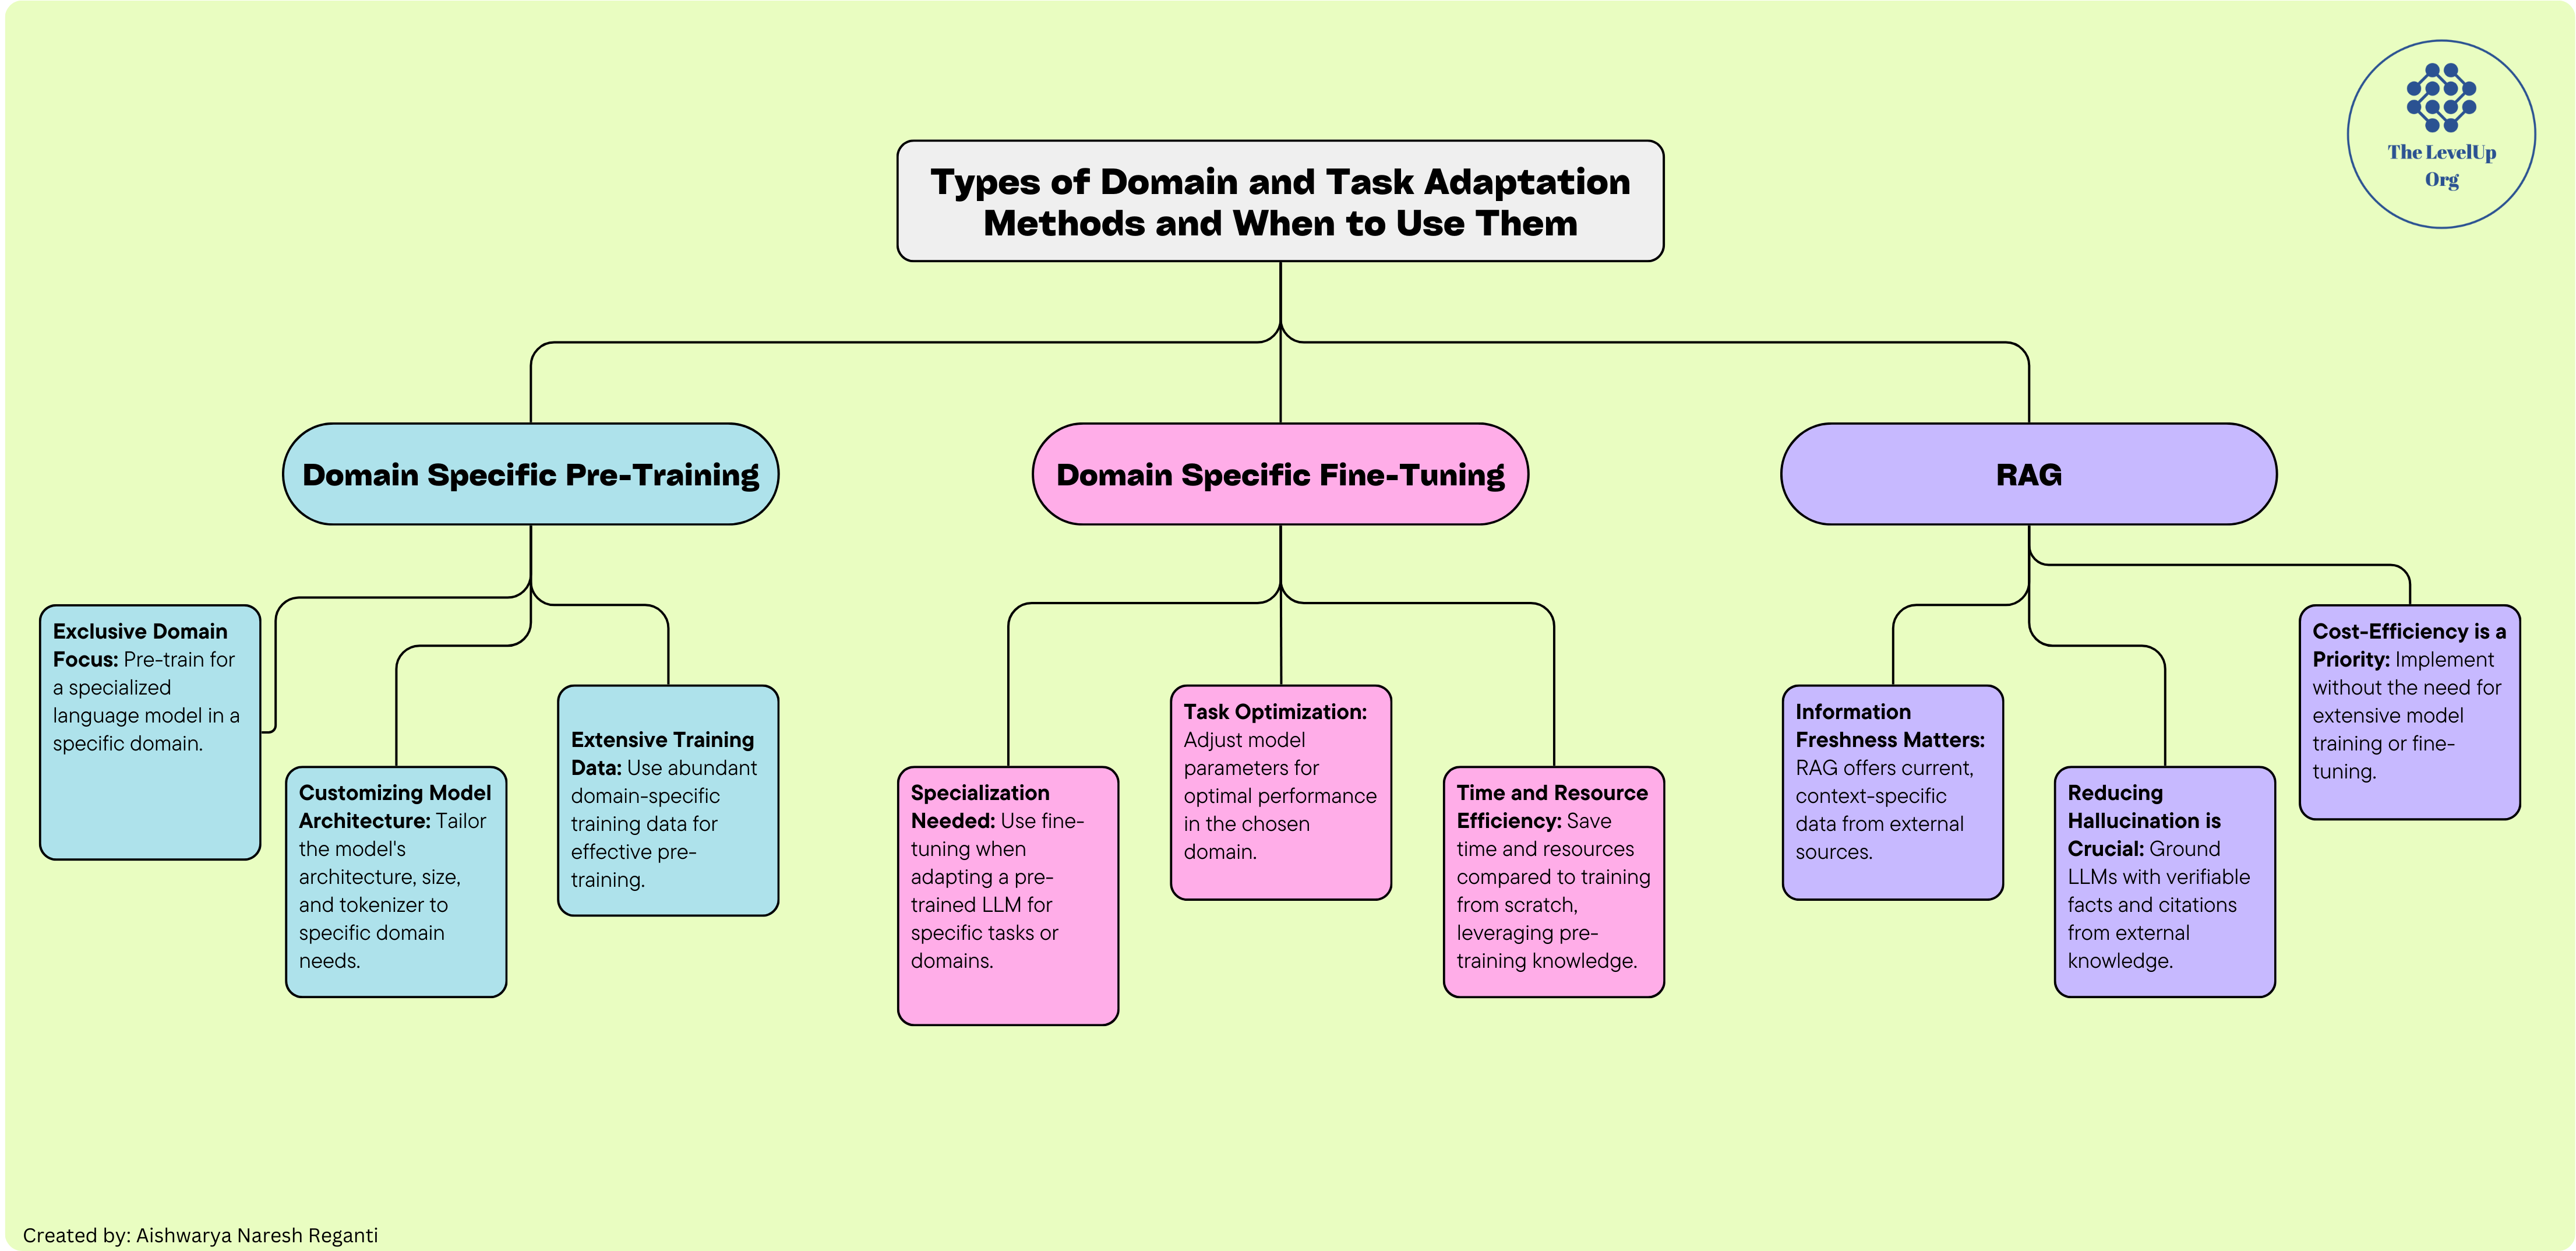
\includegraphics[width=\linewidth,keepaspectratio]{llm127}
\end{center}				

{\tiny (Ref: Applied LLMs Mastery 2024 - Aishwarya Reganti)}

\end{frame}